% Dataset construction pipeline (Stage 1) — schematic for the paper.
% Two parallel collection rails (GovInfo hearings; SEC 10-K filings) plus an
% independent human reference (C-SPAN abstracts). The stage's governing
% principle — enumerate the universe first, so every gap is a measured
% subtraction, not a later discovery — is the footer. All numbers are the
% measured counts reported in scripts/python/01_dataset_construction/.
% Compile: xelatex fig_dataset_construction.tex
\documentclass[tikz]{standalone}
\usetikzlibrary{positioning,calc,arrows.meta}

% Project palette: Royal Navy (data/flow), Deep Academic Red (measured
% defects), Muted Royal Green (stage outputs). Tints stay in these families.
\definecolor{navy}{HTML}{003049}
\definecolor{navylight}{HTML}{E8EEF2}
\definecolor{red1}{HTML}{A30006}
\definecolor{green1}{HTML}{7C9885}
\definecolor{greenlight}{HTML}{EDF2EF}
\definecolor{ink}{HTML}{2B2B2B}

\begin{document}
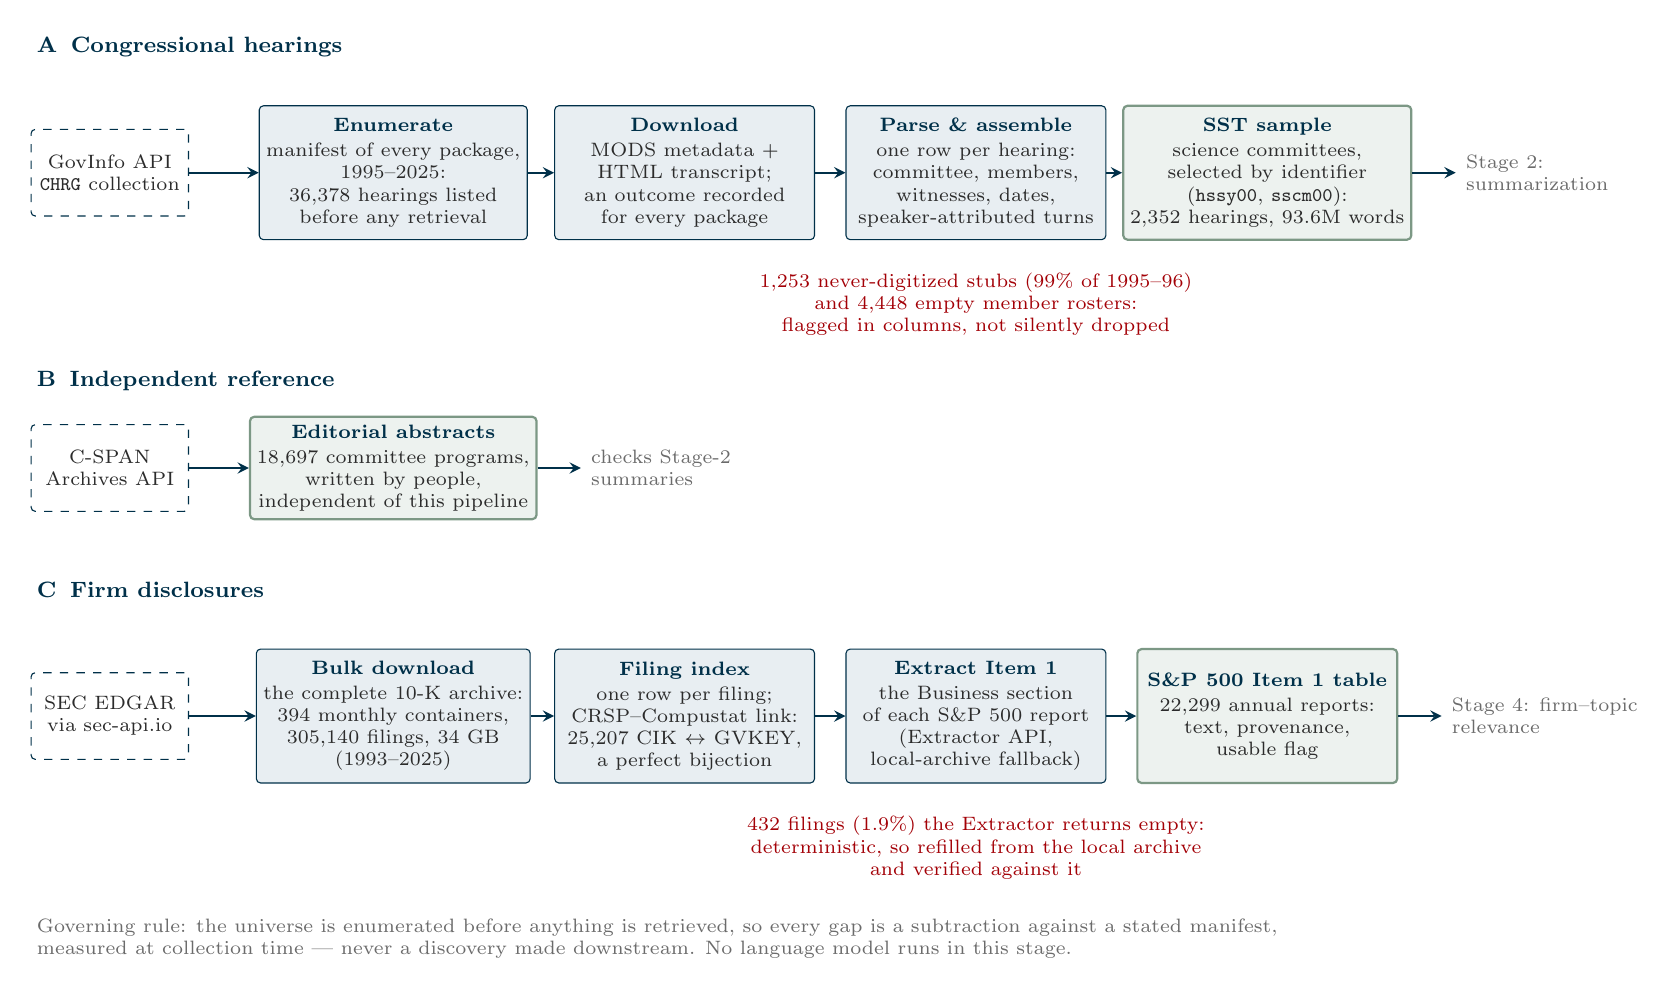
\begin{tikzpicture}[
  font=\footnotesize,
  every node/.style={text=ink},
  raillabel/.style={font=\footnotesize\bfseries, text=navy, anchor=west},
  box/.style={draw=navy, fill=navylight, rounded corners=1.5pt, align=center,
              minimum width=33mm, minimum height=17mm, inner sep=2.5pt,
              font=\scriptsize},
  outbox/.style={draw=green1, thick, fill=greenlight, rounded corners=1.5pt,
                 align=center, minimum width=33mm, minimum height=17mm,
                 inner sep=2.5pt, font=\scriptsize},
  src/.style={draw=navy, dashed, fill=white, rounded corners=1.5pt,
              align=center, minimum width=20mm, minimum height=11mm,
              inner sep=2pt, font=\scriptsize},
  head/.style={font=\scriptsize\bfseries, text=navy},
  gap/.style={font=\scriptsize, text=red1, align=center},
  note/.style={font=\scriptsize, text=ink!70, align=center},
  flow/.style={-{stealth}, navy, thick},
]

% ============================================================ hearing rail
\node[raillabel] at (-2.05,4.6) {A\enspace Congressional hearings};

\node[src] (govinfo) at (-1.0,3.0) {GovInfo API\\\texttt{CHRG} collection};

\node[box] (a1) at (2.6,3.0)
  {\textbf{\textcolor{navy}{Enumerate}}\\[1pt]
   manifest of every package,\\1995--2025:\\36{,}378 hearings listed\\before any retrieval};
\node[box] (a2) at (6.3,3.0)
  {\textbf{\textcolor{navy}{Download}}\\[1pt]
   MODS metadata +\\HTML transcript;\\an outcome recorded\\for every package};
\node[box] (a3) at (10.0,3.0)
  {\textbf{\textcolor{navy}{Parse \& assemble}}\\[1pt]
   one row per hearing:\\committee, members,\\witnesses, dates,\\speaker-attributed turns};
\node[outbox] (a4) at (13.7,3.0)
  {\textbf{\textcolor{navy}{SST sample}}\\[1pt]
   science committees,\\selected by identifier\\(\texttt{hssy00}, \texttt{sscm00}):\\
   2{,}352 hearings, 93.6M words};

\draw[flow] (govinfo.east) -- (a1.west);
\draw[flow] (a1.east) -- (a2.west);
\draw[flow] (a2.east) -- (a3.west);
\draw[flow] (a3.east) -- (a4.west);
\draw[flow] (a4.east) -- ++(0.55,0)
  node[anchor=west, note, align=left] {Stage 2:\\summarization};

\node[gap, anchor=north] at (10.0,1.85)
  {1{,}253 never-digitized stubs (99\% of 1995--96)\\
   and 4{,}448 empty member rosters:\\flagged in columns, not silently dropped};

% ============================================================ reference rail
\node[raillabel] at (-2.05,0.35) {B\enspace Independent reference};

\node[src] (cspan) at (-1.0,-0.75) {C-SPAN\\Archives API};
\node[outbox, minimum height=13mm] (b1) at (2.6,-0.75)
  {\textbf{\textcolor{navy}{Editorial abstracts}}\\[1pt]
   18{,}697 committee programs,\\written by people,\\independent of this pipeline};
\draw[flow] (cspan.east) -- (b1.west);
\draw[flow] (b1.east) -- ++(0.55,0)
  node[anchor=west, note, align=left] {checks Stage-2\\summaries};

% ============================================================ SEC rail
\node[raillabel] at (-2.05,-2.3) {C\enspace Firm disclosures};

\node[src] (edgar) at (-1.0,-3.9) {SEC EDGAR\\via sec-api.io};

\node[box] (c1) at (2.6,-3.9)
  {\textbf{\textcolor{navy}{Bulk download}}\\[1pt]
   the complete 10-K archive:\\394 monthly containers,\\305{,}140 filings, 34 GB\\(1993--2025)};
\node[box] (c2) at (6.3,-3.9)
  {\textbf{\textcolor{navy}{Filing index}}\\[1pt]
   one row per filing;\\CRSP--Compustat link:\\25{,}207 CIK $\leftrightarrow$ GVKEY,\\a perfect bijection};
\node[box] (c3) at (10.0,-3.9)
  {\textbf{\textcolor{navy}{Extract Item 1}}\\[1pt]
   the Business section\\of each S\&P 500 report\\(Extractor API,\\local-archive fallback)};
\node[outbox] (c4) at (13.7,-3.9)
  {\textbf{\textcolor{navy}{S\&P 500 Item 1 table}}\\[1pt]
   22{,}299 annual reports:\\text, provenance,\\usable flag};

\draw[flow] (edgar.east) -- (c1.west);
\draw[flow] (c1.east) -- (c2.west);
\draw[flow] (c2.east) -- (c3.west);
\draw[flow] (c3.east) -- (c4.west);
\draw[flow] (c4.east) -- ++(0.55,0)
  node[anchor=west, note, align=left] {Stage 4: firm--topic\\relevance};

\node[gap, anchor=north] at (10.0,-5.05)
  {432 filings (1.9\%) the Extractor returns empty:\\
   deterministic, so refilled from the local archive\\and verified against it};

% ============================================================ footer
\node[note, anchor=north west, align=left] at (-2.05,-6.35)
  {Governing rule: the universe is enumerated before anything is retrieved, so every gap is a
   subtraction against a stated manifest,\\measured at collection time --- never a discovery made
   downstream. No language model runs in this stage.};

\end{tikzpicture}
\end{document}
